
\documentclass{article}
\usepackage[utf8]{inputenc}
\usepackage{amsmath}
\usepackage{graphicx}
\usepackage{hyperref}

\title{Optimizing Peer Decisions in BitTorrent Networks Through Game Theory and Reinforcement Learning}
\author{Shlok Kumar Shaw \and Deshmukh Ajinkya Rajesh \and Aniket Roy \\ \textit{Supervised by: Dr. Sudipta Saha and Mr. Indrojit Dhe Shaon}}
\date{25th April 2024}

\begin{document}

\maketitle

\begin{abstract}
This paper explores the application of game theory and reinforcement learning to enhance decision-making processes in BitTorrent networks, focusing on the choking and unchoking mechanisms. By simulating various strategies within a controlled environment, we analyze the potential for these advanced methodologies to improve network efficiency and fairness compared to traditional approaches.
\end{abstract}

\section{Literature Survey}
\textbf{BitTorrent Protocol Basics:}
BitTorrent is a popular peer-to-peer (P2P) file-sharing protocol that enables efficient distribution of files across all users by breaking down files into smaller pieces, which are downloaded from multiple sources simultaneously. This decentralization eliminates the need for a powerful central server and helps handle large volumes of data while reducing bandwidth usage.
\newline
\newline
\textbf{Game Theory in BitTorrent Protocol:}
\begin {itemize} 
\item Qiu and Srikant (2004) in their seminal paper, "Modeling and Performance Analysis of BitTorrent-Like Peer-to-Peer Networks", use game theory to analyze the strategies of peers in a torrent. They propose a fluid model to describe the evolution of the system and show how game theory can explain the emergence of cooperation among peers.

\item Locher et al. (2006) explore the application of game theory to develop a mechanism that can effectively discourage selfish behavior in BitTorrent networks. Their work, "The Strongest Link: Legitimizing the Fair Use Doctrine in Peer-to-Peer Content Distribution", demonstrates how modified BitTorrent protocols can ensure fair sharing.

\end {itemize}
\textbf{Application of Reinforcement Learning in BitTorrent:}
\begin {itemize}
\item
Li et al. (2008) present a reinforcement learning framework for BitTorrent-like systems in their work, "Towards a Trustworthy Service Provision Model with a Reinforcement Learning Approach in a Peer-to-Peer Environment". They develop an algorithm that dynamically adjusts unchoking decisions based on past interactions, significantly improving download speeds and cooperation levels among peers.

\item
Magharei et al. (2009), in "Prime: Peer-to-Peer Receiver-Driven Mesh-Based Streaming", apply reinforcement learning to optimize streaming in P2P networks, adjusting the data delivery paths in real time based on network conditions. Although focused on streaming, the methods are applicable to BitTorrent-like file sharing.

\end {itemize}
These studies provide a solid foundation for integrating game theory and machine learning into the BitTorrent protocol to improve peer decision-making. They highlight both theoretical and practical considerations and show a path forward for enhancing protocol efficiency and fairness through strategic modeling and learning algorithms.

\section{Problem Definition}
\textbf{Problem Background:}
BitTorrent, a peer-to-peer (P2P) file-sharing protocol, relies on decentralized network architecture to distribute data. A core mechanism within this protocol is the decision-making process related to "choking" and "unchoking," where peers decide which other peers to send data to (unchoking) or restrict data from (choking). These decisions are crucial as they determine the efficiency and fairness of data distribution among users. Traditionally, these decisions are based on fixed heuristics that often do not adapt dynamically to changing network conditions or peer behavior.
\newline
\newline
\textbf{Current Limitations:}
\begin {itemize}
\item
Static Decision-Making: Existing heuristics in BitTorrent are rigid and often cannot effectively adapt to dynamic network environments or diverse peer strategies, leading to suboptimal data distribution and potential system inefficiencies.
\item
Inefficiency and Unfairness: Fixed algorithms may lead to scenarios where resource distribution is not optimal, causing slower download speeds for some peers and allowing others to benefit disproportionately, which can encourage free-riding and other forms of selfish behavior.
\item
Lack of Adaptability: The current protocols do not incorporate learning from past interactions, which limits the system’s ability to improve its performance over time based on empirical data.
\end {itemize}
\textbf{Proposed Research Problem:}
The aim of this research is to develop an adaptive decision-making framework within the BitTorrent protocol by modeling peer interactions as a game theoretical problem and applying reinforcement learning algorithms. This approach will enable the system to dynamically adjust its strategies based on ongoing peer behavior and network conditions.
\newline
\newline
\textbf{Objectives:}
\begin {itemize}
\item
Model Peer Interactions: Utilize game theory to model the strategic interactions between peers, focusing on the utility functions that influence their decisions to choke or unchoke others.
\item
Apply Machine Learning: Develop and implement a reinforcement learning algorithm that can learn optimal unchoking strategies based on historical data and real-time feedback from the network.
\item
Dynamic Adaptation: Create a system that dynamically adapts its strategies to maximize overall network performance and fairness, thus improving download speeds and reducing inefficiencies.
\item
Evaluation and Comparison: Assess the performance of the proposed system against traditional heuristics and measure improvements in terms of efficiency, fairness, and adaptability.
\end {itemize}
\textbf{Significance:}
This research will contribute to the understanding of decentralized network protocols by introducing a flexible, learning-based approach to decision-making in BitTorrent. By enhancing the protocol’s efficiency and fairness, the study aims to provide a more robust, scalable, and user-friendly P2P file-sharing environment.

\section{Design and Implementation}

\subsection{Simulation Environment Setup (bit.py)}
The basic BitTorrent simulation, implemented in \texttt{bit.py}, serves as the foundational model for our experiments. Here are the specific components and parameters:

\subsubsection{Peers}
Each peer in the simulation represents a node in the BitTorrent network. Peers have attributes such as a list of files they wish to download, their current inventory of file pieces, and their upload and download speeds.

\subsubsection{Files and Pieces}
Files are divided into pieces, and peers need to collect all pieces of a file to complete a download. Pieces are uniformly sized, which simplifies the tracking and exchange of file segments among peers.

\subsubsection{Network Characteristics}
\begin{itemize}
    \item \textbf{Latency:} Simulates the delay in communication between peers.
    \item \textbf{Bandwidth:} Defines the maximum upload and download capacity for each peer, affecting how quickly they can send and receive file pieces.
\end{itemize}

\subsubsection{Choking/Unchoking Mechanism}
Based on traditional heuristics, such as preferring to unchoke peers from whom a peer has recently downloaded successfully (reciprocity) and occasionally rotating peers to discover better connections (optimistic unchoking).

\subsubsection{Events}
\begin{itemize}
    \item \textbf{Piece Request:} Peers request pieces from others based on their current needs and the pieces available from their peers.
    \item \textbf{Piece Transfer:} Occurs when an unchoked peer sends a piece to another peer.
    \item \textbf{Choking Decisions:} Regular intervals where peers evaluate whom to choke or unchoke based on their strategies.
\end{itemize}

\subsection{Reinforcement Learning Model (rl.py)}
\subsubsection{Training the RL Agent}
The reinforcement learning (RL) model in our BitTorrent simulation is designed to optimize the decisions each peer makes regarding whom to choke or unchoke. The RL agent interacts with the simulation environment, learning from its actions based on the feedback received in the form of rewards.

\subsubsection{Model Architecture}
\begin{itemize}
    \item \textbf{Input:} The state of the network from the perspective of the peer, including data on available pieces, peer upload and download rates, and the history of pieces received.
    \item \textbf{Output:} A set of actions, specifically decisions on which peers to choke or unchoke.
\end{itemize}

\subsubsection{State Representation}
The state input to the RL model includes:
\begin{itemize}
    \item \textbf{Peer Inventory:} A binary vector indicating which pieces each connected peer possesses.
    \item \textbf{Data Rates:} Historical upload and download rates between the peer and each of its connections, providing a basis for predicting beneficial exchanges.
    \item \textbf{Recent Actions:} Recently taken actions to incorporate strategy persistence and adaptiveness.
\end{itemize}

\subsubsection{Action Space}
The action space is discrete, where each action represents a combination of choke and unchoke decisions towards other peers in the network. Given \( n \) peers, the action space grows combinatorially, which is typically managed through action reduction techniques or policy-based approaches.

\subsubsection{Reward Function}
The reward function is crucial as it guides the learning process by quantifying the desirability of the outcomes resulting from taken actions. The rewards are structured to promote:
\begin{itemize}
    \item \textbf{High Download Rates:} Rewards are proportional to the increase in download completion rates, incentivizing actions that lead to faster downloads.
    \item \textbf{Fairness:} Actions that lead to equitable resource sharing among peers are rewarded, aiming to discourage free-riding and to promote contribution to the network.
\end{itemize}

\subsubsection{Learning Process}
The reinforcement learning model is designed to optimize the decisions each peer makes regarding whom to choke or unchoke through a dynamic adjustment of strategy based on the network's state and peer actions. This process hinges on the iterative calculation of a loss function and subsequent updates to the model's parameters via backpropagation, aimed at enhancing network performance in terms of fairness and efficiency.

\paragraph{Loss Function Calculation}
The loss function quantifies the efficiency of the current strategy by evaluating the contributions of each peer based on their upload rate, uploaded pieces, and downloaded pieces. These contributions are weighted by coefficients that reflect their respective importance: the upload rate, the number of pieces uploaded, and the number of pieces downloaded. The overall loss is calculated as the sum of the contributions from all peers, adjusted for the number of uploads they completed in the last step. This adjustment serves to penalize or reward peers based on their net contribution to the network's health, thereby aligning individual incentives with overall network performance.

\paragraph{Backpropagation}
Following the loss calculation, the model's weights are updated using a backpropagation technique that adjusts the weights to minimize the loss. The gradients of the loss with respect to each weight are computed across all peers. These gradients indicate how changes in the weights affect the overall loss, guiding the updates to enhance network performance. The weights are adjusted in proportion to the gradients, scaled by a learning rate that dictates the speed of learning. This method ensures that the strategy evolves towards more effective peer interactions, promoting an equitable distribution of resources and improving the overall health and efficiency of the network.

This continuous learning process enables the model to adapt to varying network conditions and peer behaviors dynamically. By leveraging actual data from network interactions, the reinforcement learning approach not only seeks to improve immediate network performance but also aims to ensure the long-term sustainability and robustness of the BitTorrent ecosystem.

\subsection{Alternative Strategies (bit1.py, bit2.py, bit3.py)}
These scripts explore different heuristics and algorithms for managing peer interactions, providing comparative data for the RL approach.
\begin{itemize}
    \item \textbf{bit1.py:} Uses a priority queue based on upload speed to determine choking decisions.
    \item \textbf{bit2.py:} Implements an enhanced tit-for-tat strategy with added randomness to counteract potential gaming by peers.
    \item \textbf{bit3.py:} Adopts a proportional share algorithm where peers adjust their upload capacity based on observed download rates, promoting a more equitable resource distribution.
\end{itemize}

\subsection{Simulation Runs and Data Collection}
Each script is executed under controlled simulations with predefined network setups to ensure comparable results. Data collected from these simulations include metrics such as download times, upload/download ratios, number of chokes and unchokes, and overall network throughput. This data is crucial for evaluating the effectiveness of each strategy and for training and refining the reinforcement learning model.
```

This code covers the detailed explanation of the design and implementation of your simulation, focusing on the various components, parameters, and methods employed.

\newpage
\section{Simulation Results}
This section presents the results from the simulations of the five different approaches implemented in our study. Each approach is evaluated based on several key metrics: the average completion step versus upload speed histogram, the total steps taken, the median of the ratio of total uploaded pieces to total downloaded pieces, and comments on the observed outcomes.

\subsection{Vanilla BitTorrent Protocol (bit.py)}
\begin{itemize}
\item \textbf{Average Completion Step vs. Upload Speed Histogram:}

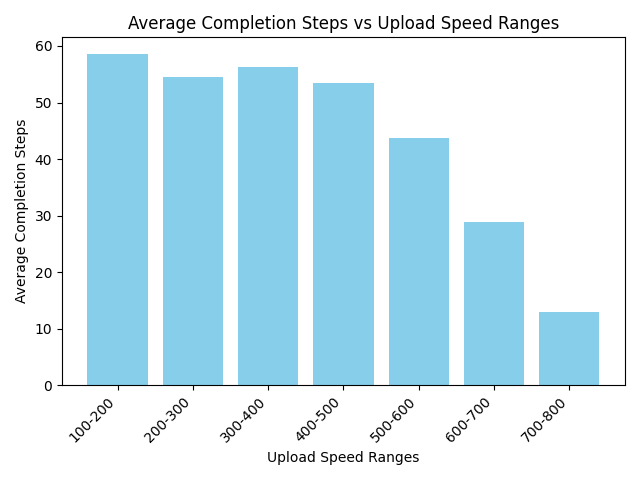
\includegraphics[width=\linewidth]{graphs/bit.png}
\item \textbf{Total Steps Taken:} 73
\item \textbf{Median of Ratio (Uploaded/Downloaded):} 0.92157
\item \textbf{Comments:} These results indicate that the traditional BitTorrent protocol performs reasonably well in terms of download completion times and fairness in resource sharing. However, there is room for improvement in optimizing upload speeds and enhancing cooperation among peers.
\end{itemize}
\newpage
\subsection{Reinforcement Learning Approach (rl.py)}
\begin{itemize}
\item \textbf{Average Completion Step vs. Upload Speed Histogram:} 

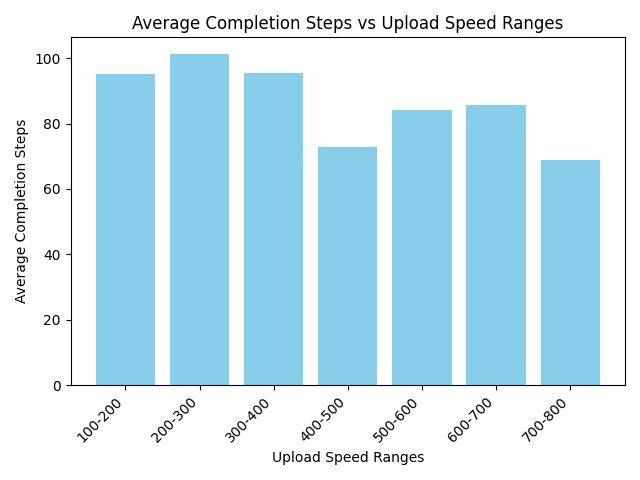
\includegraphics[width=\linewidth]{graphs/rl.png}
\item \textbf{Total Steps Taken:} 102
\item \textbf{Median of Ratio (Uploaded/Downloaded):} 0.80392
\item \textbf{Comments:} The reinforcement learning model shows promising results in terms of optimizing choking and unchoking decisions. But it falls slightly short of the vanilla BitTorrent protocol in terms of download completion times and fairness. Further tuning and training of the RL model could potentially enhance its performance.
\end{itemize}

\newpage
\subsection{Alternative Strategy 1 (bit1.py)}
\begin{itemize}
\item \textbf{Average Completion Step vs. Upload Speed Histogram:} 

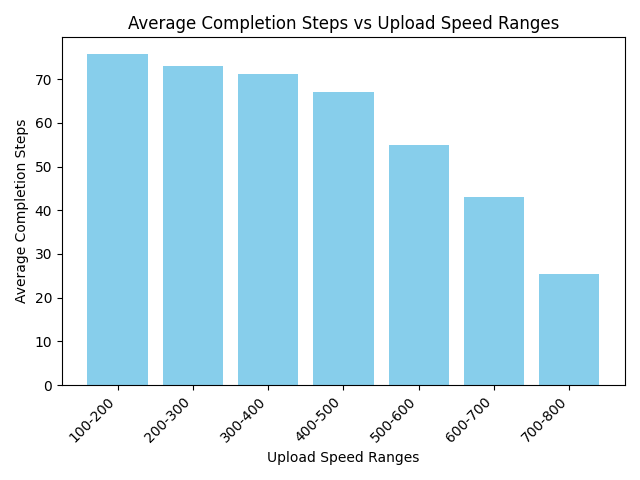
\includegraphics[width=\linewidth]{graphs/bit1.png}
\item \textbf{Total Steps Taken:} 81
\item \textbf{Median of Ratio (Uploaded/Downloaded):} 0.62745
\item \textbf{Comments:} Strategy 1 shows a significant deviation from the vanilla BitTorrent protocol, with a lower median ratio of uploaded to downloaded pieces. This suggests that dividing bandwidth greedily based on upload speed may not be the most effective approach for optimizing network performance and fairness.
\end{itemize}

\newpage
\subsection{Alternative Strategy 2 (bit2.py)}
\begin{itemize}
\item \textbf{Average Completion Step vs. Upload Speed Histogram:} 

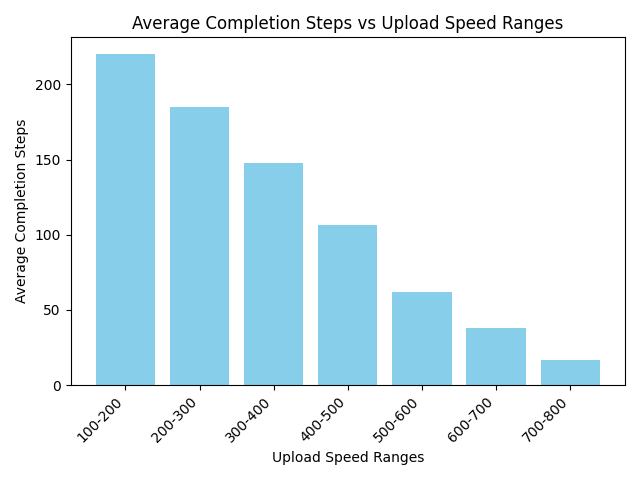
\includegraphics[width=\linewidth]{graphs/bit2.png}
\item \textbf{Total Steps Taken:} 225
\item \textbf{Median of Ratio (Uploaded/Downloaded):} 0.60784
\item \textbf{Comments:} Strategy 2 exhibits a more erratic completion step distribution compared to the vanilla BitTorrent protocol. This suggests that making reciprocity optional may not be conducive to network efficiency and fairness.
\end{itemize}

\newpage
\subsection{Alternative Strategy 3 (bit3.py)}
\begin{itemize}
\item \textbf{Average Completion Step vs. Upload Speed Histogram:} 

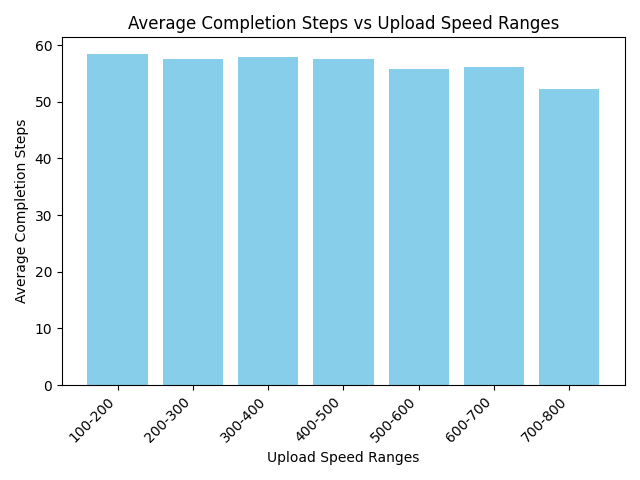
\includegraphics[width=\linewidth]{graphs/bit3.png}
\item \textbf{Total Steps Taken:} 59
\item \textbf{Median of Ratio (Uploaded/Downloaded):} 0.72549
\item \textbf{Comments:} Strategy 3 adopts a radical approach to resource sharing, adjusting upload capacity based on resource availability, while ignoring fairness. This results in a lower median ratio of uploaded to downloaded pieces, but faster overall resource distribution as indicated by the low total steps taken. Its performance highlights the trade-offs between fairness and efficiency in P2P networks.
\end{itemize}


\section{Conclusion}
In this study, we have explored the application of reinforcement learning to optimize decision-making in the BitTorrent protocol, specifically focusing on the choking and unchoking mechanisms that significantly impact the efficiency and fairness of the network. Our implementation involved developing a simulation environment where various strategies, including a reinforcement learning (RL) model, were tested against traditional BitTorrent heuristics.

The results from our simulations indicate that the RL-based approach, while slightly underperforming in comparison to the vanilla BitTorrent protocol under the controlled conditions of our experiment, holds considerable promise for real-world applications. In our simulated environment, the parameters, such as upload speeds and the number of files shared, were kept constant. However, real-world P2P networks are characterized by their dynamic nature where multiple files are shared simultaneously, and the upload capacities of peers can vary significantly over time.

We believe that the RL model's ability to learn and adapt based on historical data and ongoing network interactions can offer substantial improvements in network fairness. The RL approach is particularly adept at recognizing and rewarding peers based on their contribution history, not just their instantaneous upload capacity. This feature is crucial in real-world scenarios where network conditions and peer capabilities are continually changing. By effectively recognizing and compensating peers with a consistent history of good contributions, even if their current upload speeds are momentarily low, the RL model promotes a more cooperative and fair network environment.

Such dynamic adaptability ensures that the network remains robust against fluctuations and can provide consistent performance improvements over time. Therefore, while our initial results show a slight lag behind traditional methods in a controlled test environment, the adaptive and predictive capabilities of the RL model are expected to deliver superior performance in more complex, realistic settings.

In conclusion, the reinforcement learning-based approach to managing choking and unchoking decisions in BitTorrent-like networks offers a promising avenue for future research and development, potentially leading to significant enhancements in both the efficiency and fairness of peer-to-peer file-sharing networks. Further research, involving more varied simulation conditions and extended testing scenarios, will be crucial in refining the model and fully realizing its potential in practical applications.

\section{Source Code}
The source code for all simulations and strategies discussed in this paper is available at the GitHub repository \href{https://github.com/shlok-007/CN-Lab-Project}{here}. We encourage readers to explore the code, run their experiments, and contribute to the ongoing development of this research project.

\section{References}
\begin{enumerate}
\item Qiu, L., \& Srikant, R. (2004). Modeling and performance analysis of BitTorrent-like peer-to-peer networks.
\item Locher, T., Mihail, M., \& Wattenhofer, R. (2006). The strongest link: Legitimizing the fair use doctrine in peer-to-peer content distribution.
\item Li, B., \& Li, J. (2008). Towards a trustworthy service provision model with a reinforcement learning approach in a peer-to-peer environment.
\item Magharei, N., \& Rejaie, R. (2009). Prime: Peer-to-peer receiver-driven mesh-based streaming.

\end{enumerate}

\end{document}
